
% !TEX root = ../main.tex

% Local Variables:
% TeX-master: "../main"
% End:
% chktex-file 26

%%%%%%%%%%%%%%%%%%%%%%%%%%%%%%% Header %%%%%%%%%%%%%%%%%%%%%%%%%%%%%%%%%%%%%%%%%%%%
\begin{minipage}[l]{0.42\textwidth}
    \includegraphics[width=1\textwidth]{img/logo-UNAMBA.png}
\end{minipage}
\hfill
\begin{minipage}[c]{0.5\textwidth}
    \begin{flushright}
	\large{\textbf{Unidad \#1}}\\
	\large{Lectures on Física III}\\
	\large{24 de Septiembre del 2025. Haquira, Apurimac}\\
        % \large{\textbf{Student:} Huallpa Aimituma Josué David}
    \end{flushright}
\end{minipage}
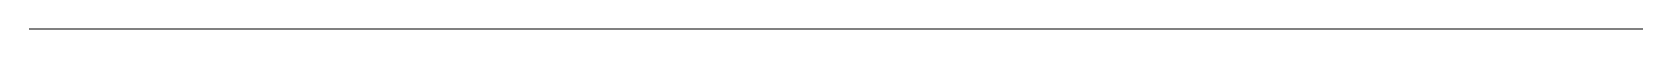
\begin{tikzpicture}
    \draw[gray,thick] (-6.5,0)--(14,0);
\end{tikzpicture}


 %%%%%%%%%%%%%%%%%%%%%%%% INICIO DEL CONTENIDO EN DOS COLUMNAS %%%%%%%%%%%%%%%%%%%%%
  
 \begin{multicols}{2}
   \begin{center}
         \LARGE{\textbf{Capítulo I: Electrostática}}\\	
         \vspace{0.2cm}
         % \Large {Lecturers Esteban Chalbaud \& Daniel Galviz} \\
         % \large{Teaching Assistant: Mauricio Gamonal \& Irvin Martínez}\\
         % \large{PhysicsLatam.com}\\
         % \vspace{0.2cm}
         \large{24 Septiembre 2025, 6:59 am (GMT-4)}\\
         % \vspace{0.2cm}
         \large{— Ficha de Trabajo —}
     \end{center}
    %%%%%%%%%%%%%%%%%%%%%%%%%%%%excercise%%%%%%%%%%%%%%%%%%%%%%%%%%%%%%%%%%%%%%%%
    \begin{excercise}[][][$Q=44.68\, \rm{\mu C}$]{ex:k28}{
        Una esfera de 2 cm de radio contiene una densi
        dad de carga por unidad de volumen $\rho_v$ que se de
        termina mediante 
        \begin{equation}
            \rho_v=4\cos^2(\theta)
        \end{equation}
         Calcule la carga total $Q$ contenida en la esfera.
         }
    \end{excercise}


\end{multicols}
